% brujula-rosa.tex — ROSA DE LOS VIENTOS de la cápsula #2 (serie "La economía son ideas").
% Rosa náutica clásica dibujada de verdad (TikZ + EB Garamond): estrella de 8 puntas
% con mitades llenas/huecas, 32 rumbos de portulano, graduación fina y N·E·S·O.
% Tinta negra sobre blanco: el shader del compás la usa como MÁSCARA — las marcas
% se vuelven ORO grabado sobre laca oscura, y la N flamea cuando la aguja clava el norte.
%   pdflatex → pdftoppm -png -r 600 → public/textures/brujula-rosa.png
\documentclass[tikz]{standalone}
\usepackage[T1]{fontenc}
\usepackage{ebgaramond}
\begin{document}
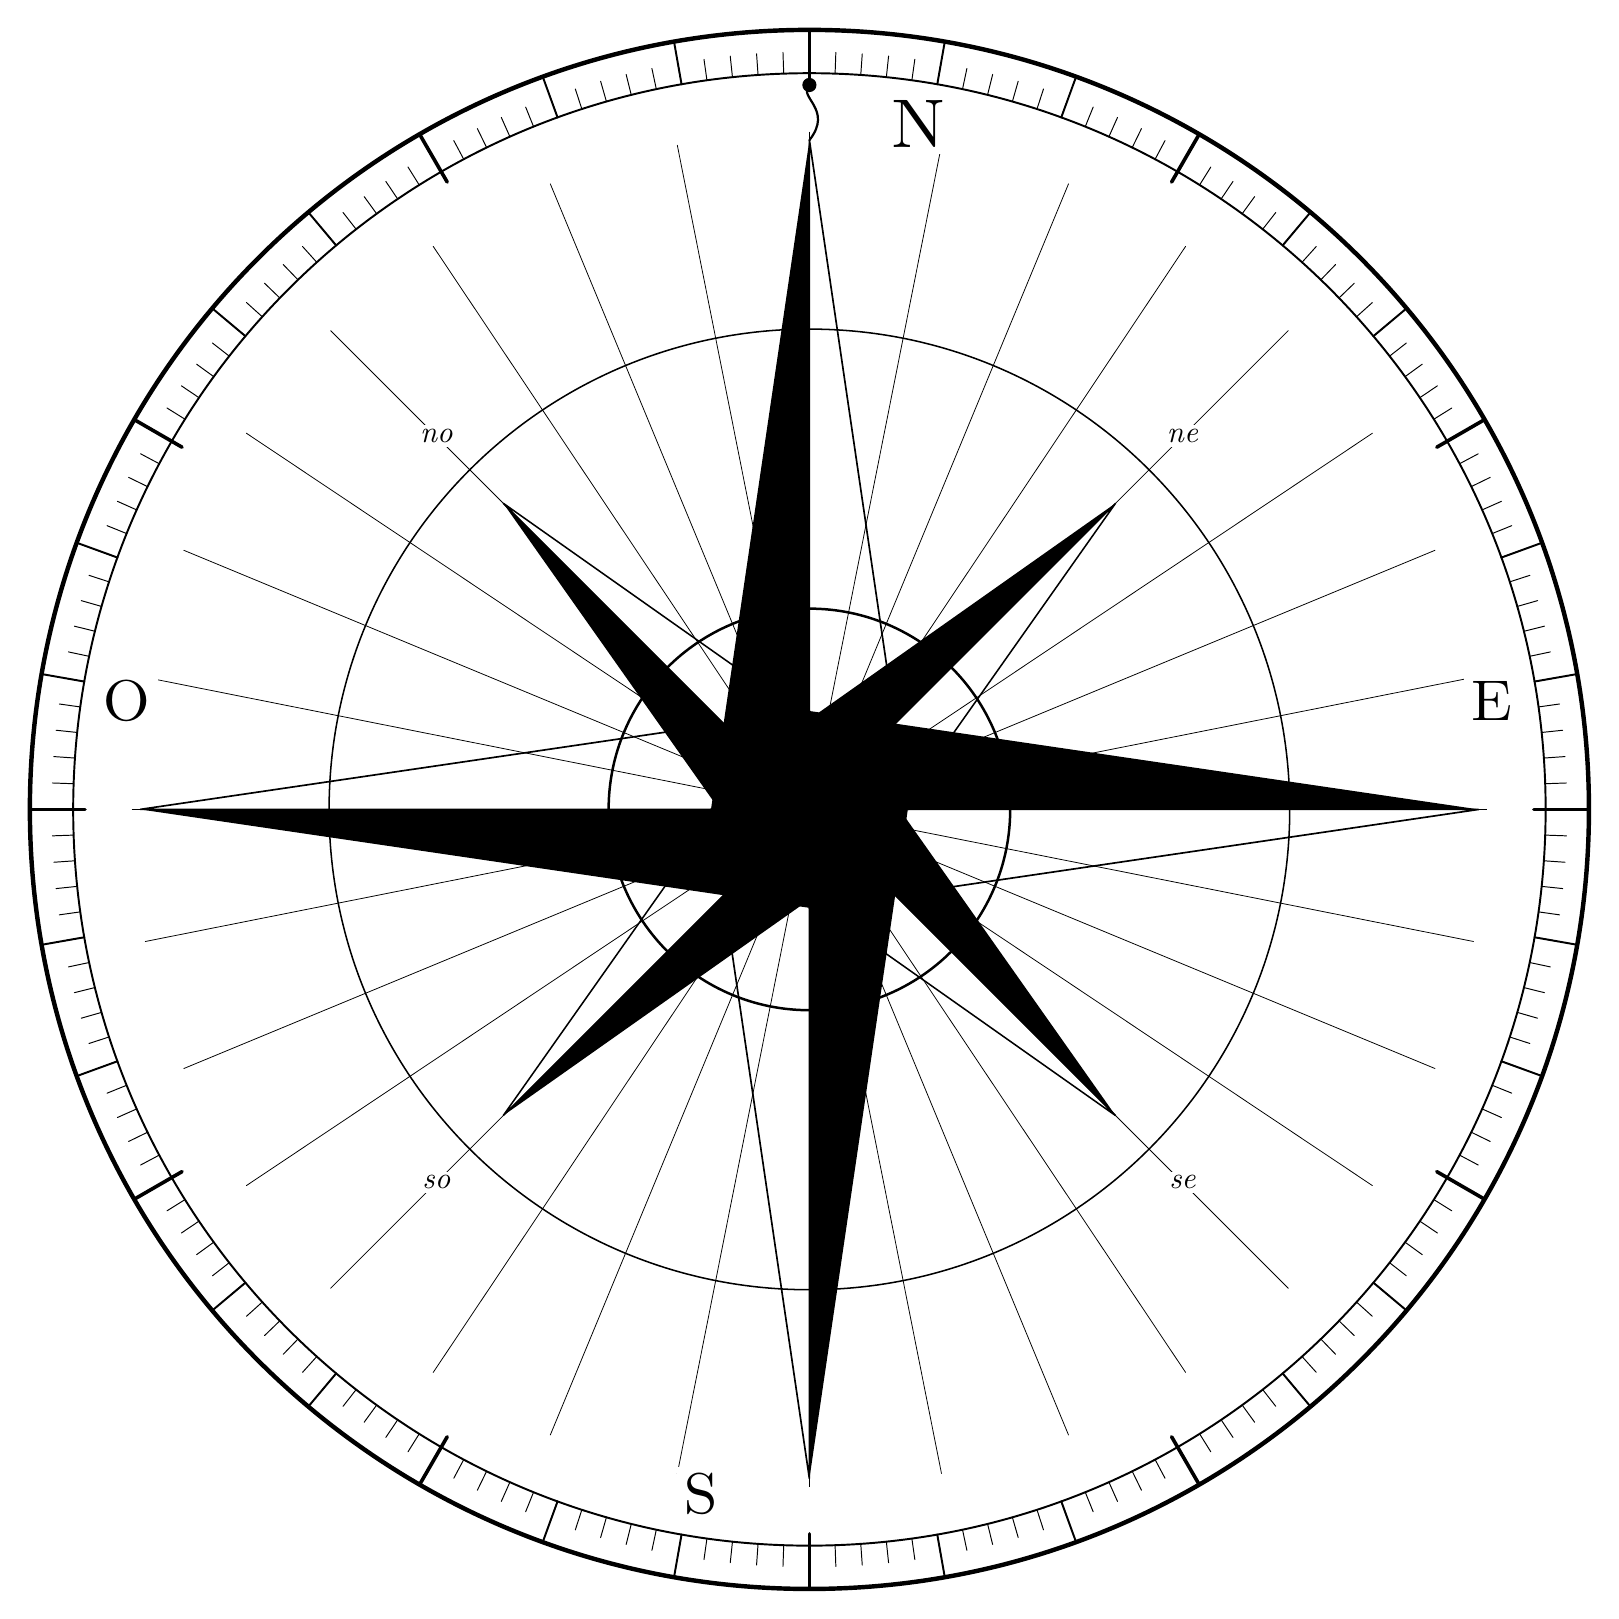
\begin{tikzpicture}[line cap=round]
  % ── anillo exterior con graduación ──
  \draw[line width=1.6pt] (0,0) circle (9.9);
  \draw[line width=0.7pt] (0,0) circle (9.35);
  \foreach \a in {0,2,...,358} { \draw[line width=0.35pt] (\a:9.35) -- (\a:9.62); }
  \foreach \a in {0,10,...,350} { \draw[line width=0.7pt] (\a:9.35) -- (\a:9.9); }
  \foreach \a in {0,30,...,330} { \draw[line width=1.3pt] (\a:9.2) -- (\a:9.9); }
  % ── 32 rumbos de portulano (rayos finos) ──
  \foreach \a in {0,11.25,...,348.75} { \draw[line width=0.28pt] (0,0) -- (\a:8.6); }
  % ── círculos interiores ──
  \draw[line width=0.55pt] (0,0) circle (6.1);
  \draw[line width=0.9pt] (0,0) circle (2.55);
  % ── estrella: 8 medias puntas LLENAS (lado horario) + 8 huecas (contorno) ──
  % intercardinales (cortas, r=5.5) DEBAJO de las cardinales
  \foreach \a in {45,135,225,315} {
    \fill (\a:5.5) -- (\a+90:0.95) -- (0,0) -- cycle;
    \draw[line width=0.55pt] (\a:5.5) -- (\a-90:0.95) -- (0,0) -- cycle;
  }
  % cardinales (largas, r=8.5)
  \foreach \a in {90,0,180,270} {
    \fill (\a:8.5) -- (\a+90:1.25) -- (0,0) -- cycle;
    \draw[line width=0.6pt] (\a:8.5) -- (\a-90:1.25) -- (0,0) -- cycle;
  }
  % ── pivote central ──
  \fill (0,0) circle (0.34);
  \draw[line width=0.6pt] (0,0) circle (0.62);
  % ── letras cardinales: en el CLARO entre las puntas (r=8.5) y el anillo (9.35),
  %    desplazadas 9° del eje para no chocar con la punta; placa blanca detrás
  %    (en la máscara blanco = fondo del disco → la letra respira) ──
  \node[fill=white, inner sep=2.5pt] at (81:8.82)  {\fontsize{26}{26}\selectfont\scshape N};
  \node[fill=white, inner sep=2.5pt] at (9:8.78)   {\fontsize{21}{21}\selectfont\scshape E};
  \node[fill=white, inner sep=2.5pt] at (261:8.8)  {\fontsize{21}{21}\selectfont\scshape S};
  \node[fill=white, inner sep=2.5pt] at (171:8.78) {\fontsize{21}{21}\selectfont\scshape O};
  % ── intercardinales chicas ──
  \node[fill=white, inner sep=1.6pt] at (45:6.7)  {\fontsize{11}{11}\selectfont\itshape ne};
  \node[fill=white, inner sep=1.6pt] at (135:6.7) {\fontsize{11}{11}\selectfont\itshape no};
  \node[fill=white, inner sep=1.6pt] at (225:6.7) {\fontsize{11}{11}\selectfont\itshape so};
  \node[fill=white, inner sep=1.6pt] at (315:6.7) {\fontsize{11}{11}\selectfont\itshape se};
  % ── flor de lis apuntando al norte (tradición portulana, sencilla) ──
  \draw[line width=0.8pt] (90:8.5) .. controls (88:8.9) and (91:9.05) .. (90:9.2);
  \fill (90:9.2) circle (0.09);
\end{tikzpicture}
\end{document}
